\documentclass[a4paper, 11pt]{scrreprt}

\usepackage{german}
\usepackage{float}
\usepackage{graphicx} 

\usepackage[margin=25mm,right=25mm, left=25mm]{geometry}


\author{Timo Schwertfeger, Daniel Kaiser, Patrick Preu"s}

\title{Dokumentation f"ur das Softwaretechnik-Projekt AppCiMo (application for city movement) 
\newline
\newline
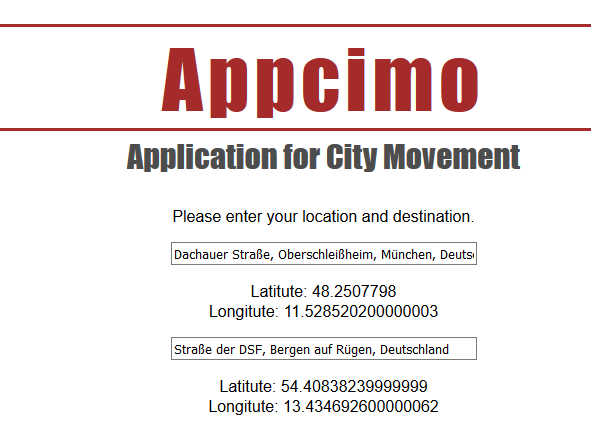
\includegraphics[width=0.7\textwidth]{appcimo.png}}



\begin{document}

\maketitle

\setcounter{secnumdepth}{5}
\setcounter{tocdepth}{5}

\tableofcontents


\chapter{Einleitung}

\section{Ausgangssituation}

\section{Zielsetzung}

\chapter{Projektvorbereitung}

\section{Projektmanagementsoftware Taiga.io}

\subsection{Vorgehensmodell}

\subsection{Einrichtung Taiga.io}

\subsection{Definition von User-Stories}

\subsection{Definition von Tasks}

\subsection{Integration HipChat}

\section{Projektdurchführung}

\subsection{Sprintplanung}

\subsection{Retrospektive}

\chapter{Pflichtenheft}

\section{Produktanforderungen}

\subsection{funktionale Anforderungen}

\begin{table}[h]

\caption{funktionale Anforderungen}

\ \\

\par

\label{tab:Tabelle1}

\centering

\begin{tabular}{|p{2.5cm} p{12cm}| ll}

\hline

Nr.	& Beschreibung\\

\hline

FU01 &	Das System muss f"ahig sein JSON-Objekte aus den Anfragen an die Google API zu verarbeiten.\\

\hline
FU02 &	Sobald der Benutzer eine Verbindung sucht, muss das System dem Benutzer die M"oglichkeit bieten einen Start- und Zielort einzugeben.\\

\hline
FU03& Sobald der Benutzer den Start- und Zielort eingibt, muss das System die Möglichkeit bieten, dem Benutzer eine Vorschlagsliste während der Eingabe anzuzeigen.\\

\hline
FU03.01	&Die Vorschlagsliste muss bei der Eingabe des ersten Zeichens angezeigt werden.\\

\hline
FU03.02	&Die vorgeschlagenen Tupel sollen mit folgender Reihenfolge angezeigt werden, 1. Straße, 2. Ort, 3. Postleitzahl\\

\hline
FU04	&Sobald der Benutzer Start und Zielort eigegeben hat, muss das System die Möglichkeit bieten, die gesuchte Verbindung mit unterschiedlichen Transportmitteln anzuzeigen.\\

\hline
FU04.01	&Das Transportmittel „zu Fuß“ muss auswählbar sein.\\

\hline
FU04.02&	Das Transportmittel  „Auto“ muss auswählbar sein.\\

\hline
FU04.03	&Das Transportmittel „öffentliche Verkehrsmittel“ muss auswählbar sein.\\

\hline
FU05	&Falls der Benutzer die Suchanfrage ändert, muss das System die Möglichkeit bieten, die gesuchte Verbindung und die Karte zu aktualisieren.\\

\hline
FU05.01	&Die Vorschlagsliste muss bei Neueingabe des Start- und Zielorts angezeigt werden.\\

\hline
FU05.02	&Die Verbindungskarte muss mit neuem Start- und Zielort die gesuchte Verbindung anzeigen.\\

\hline
FU05.03	&Die Distanz der neuen Verbindung muss aktualisiert werden.\\

\hline
FU05.04&	Die Dauer der neuen Verbindung muss aktualisiert werden.\\

\hline
FU05.05	&Der Preis der neuen Verbindung muss angezeigt werden.\\

\hline
FU06	&Falls der Benutzer eine Verbindung sucht, muss das System die Möglichkeit bieten, mehrere Transportmittel auszuwählen.\\

\hline
FU07	&Sobald der Benutzer eine Verbindung sucht, muss das System die Möglichkeit bieten, eine Ergebnisliste der gesuchten Verbindung anzuzeigen.\\

\hline
FU07.01&	In der Ergebnisliste muss der aktuelle Preis angezeigt werden.\\

\hline
FU07.02 &	In der Ergebnisliste muss die Dauer angezeigt werden.\\

\hline
FU07.03&	In der Ergebnisliste muss die Distanz angezeigt werden.\\

\hline


\end{tabular}

\end{table}

\subsection{Nicht-funktionale Anforderungen}

\begin{table}[h]

\caption{Projektanforderungen}

\ \\

\par

\label{tab:Tabelle1}

\centering

\begin{tabular}{|p{2.5cm} p{12cm}| ll}

\hline
Nr.	& Beschreibung\\

\hline
NFU01 &	Das System muss plattformunabhängig und webbasiert sein. \\

\hline
NFU02 &	Das System muss mit einem Entwicklungs-Framework umgesetzt werden.\\

\hline
NFU03 &	Das System soll als Single-Page Anwendung umgesetzt werden.\\

\hline

\end{tabular}

\end{table}

\subsection{Projektanforderungen}

\begin{table}[h]

\caption{Nicht-funktionale Anforderungen}

\ \\

\par

\label{tab:Tabelle1}

\centering

\begin{tabular}{|p{2.5cm} p{12cm}| ll}

\hline
Nr. &	Beschreibung\\

\hline
PRJ01 &	Für die Umsetzung des Systems soll ein modernes Entwicklungs-Framework für die Softwareerstellung genutzt werden.\\
PRJ02 &	Es muss eine Projektmanagementsoftware, für die mit der Softwareerstellung einhergehende Projektarbeit, genutzt werden.\\

\hline
PRJ03 &	Der entwickelte Programmcode muss auf Github als Master-Branch hochgeladen werden.\\

\hline
PRJ04 &	Für das Software-Projekt muss eine Projektdokumentation erstellt werden.\\

\hline
\end{tabular}

\end{table}
\subsection{Abnahmekriterien}

\section{Konfiguration und Einrichtung zur Softwareentwicklung}

\subsection{Entwicklungsumgebung}

\subsection{VueJS}

\subsection{Node.js und NPM}

\subsection{Github}

\subsection{TravisCI}


\chapter{Systementwurf und Umsetzung}

\section{Systemkomponenten}

\subsection{Komponentendiagramm}

\subsection{Komponentenbeschreibung}

\section{Google API}

\subsection{Google Services}

\subsection{Verarbeitung JSON-Objekte}

\subsection{Methoden}

\subsection{Refactoring und Tests}

\chapter{Zusammenfassung und Ausblick}

\section{Zusammenfassung}

\section{Ausblick}

\chapter{Anhänge}

\section{Glossar}

\section{verwendete Software}













\end{document}
